\section{Note échange}
\label{theorie}
Changememnt moyen prod: renouvelable increase entraîne gaz et charbon increase, qui évoluent avec le prix du pétrole. \\

Donnée mensuelle : pas accessible. 

Co-integration: prendre des valeurs critiques. Helmut Luckte Paul. Bootstrap. 

Pesaran: optimal prediction with weighting on covid data.
 

\newpage

\section{Introduction}
As France aim to achieve carbon neutrality by 2050\footnote{see \href{https://www.legifrance.gouv.fr/jorf/id/JORFTEXT000041814459}{Légifrance}.}, it is of great matter to understand the determinants of past electricity consumption in order to predict future trends and build prospective scenarios that will inform energy policies. Despite the many reason that could explain the evolution of electricity consumption (structural changes in production and consumption, especially with regard to the energetic transition, AI consumption \cite{de2023growing}, etc.), we will keep the model simple and focus on the main determinants of electricity consumption: income, price and annual climate variations. The provided forecast therefore be seen as a potential baseline scenario, built only from what have existed, completely blind to any future changes (or crisis) in the economy.

\section{Methods}

\subsection{About the dataset}

The given dataset is composed of 6 annual time series over electricity consumption, GDP, population, inflation (through Consumer Price Index), electricity price, and a climate index. The data is available from 1990 to 2021, therefore providing 32 observations. 

We first tried to find more granular data, \textit{e.g.} quarterly one, but no source could provide electricity information over the 1990-2021 time period (the IAE has been charging for data since january 2025, Eurostat doesn't have reliable french data before 2005)\footnote{For inflation and GDP, we could have used INSEE database, \href{https://www.insee.fr/fr/statistiques/serie/001763852\#Telechargement}{here} and
\href{https://www.insee.fr/fr/statistiques/8196636?sommaire=8182908\#consulter}{there}.}. From this situation, we already know that, dealing with low-frequency data, we will not be able to include annual variability in our analysis, which could have been interesting for studying seasonal effects on electricity. We also will not be able to use moving average filter (\textit{e.g.} Hodrick-Prescott) to identify trends, economic cycles, and fluctuations in GDP.

To our available data we add the real net disposable income of households and Non-Profit Institutions Serving Households (NPISH), deflated by final consumption expenditure (expressed in millions euros 2020, chained volumes\footnote{see \href{https://data-explorer.oecd.org/vis?pg=0&snb=12&vw=tb&df[ds]=dsDisseminateFinalDMZ&df[id]=DSD_NAAG\%40DF_NAAG_V&df[ag]=OECD.SDD.NAD&df[vs]=1.0&dq=A..B6GS1M_POP..&pd=1970\%2C&to[TIME_PERIOD]=false&lb=bt&lc=fr}{OCDE}.}), the deflator being the Consumer Price Index (CPI). Because it captures changes in household market purchasing power, it might be a better proxy for an income effect on electricity consumption.

\begin{figure}[h]
    \centering
      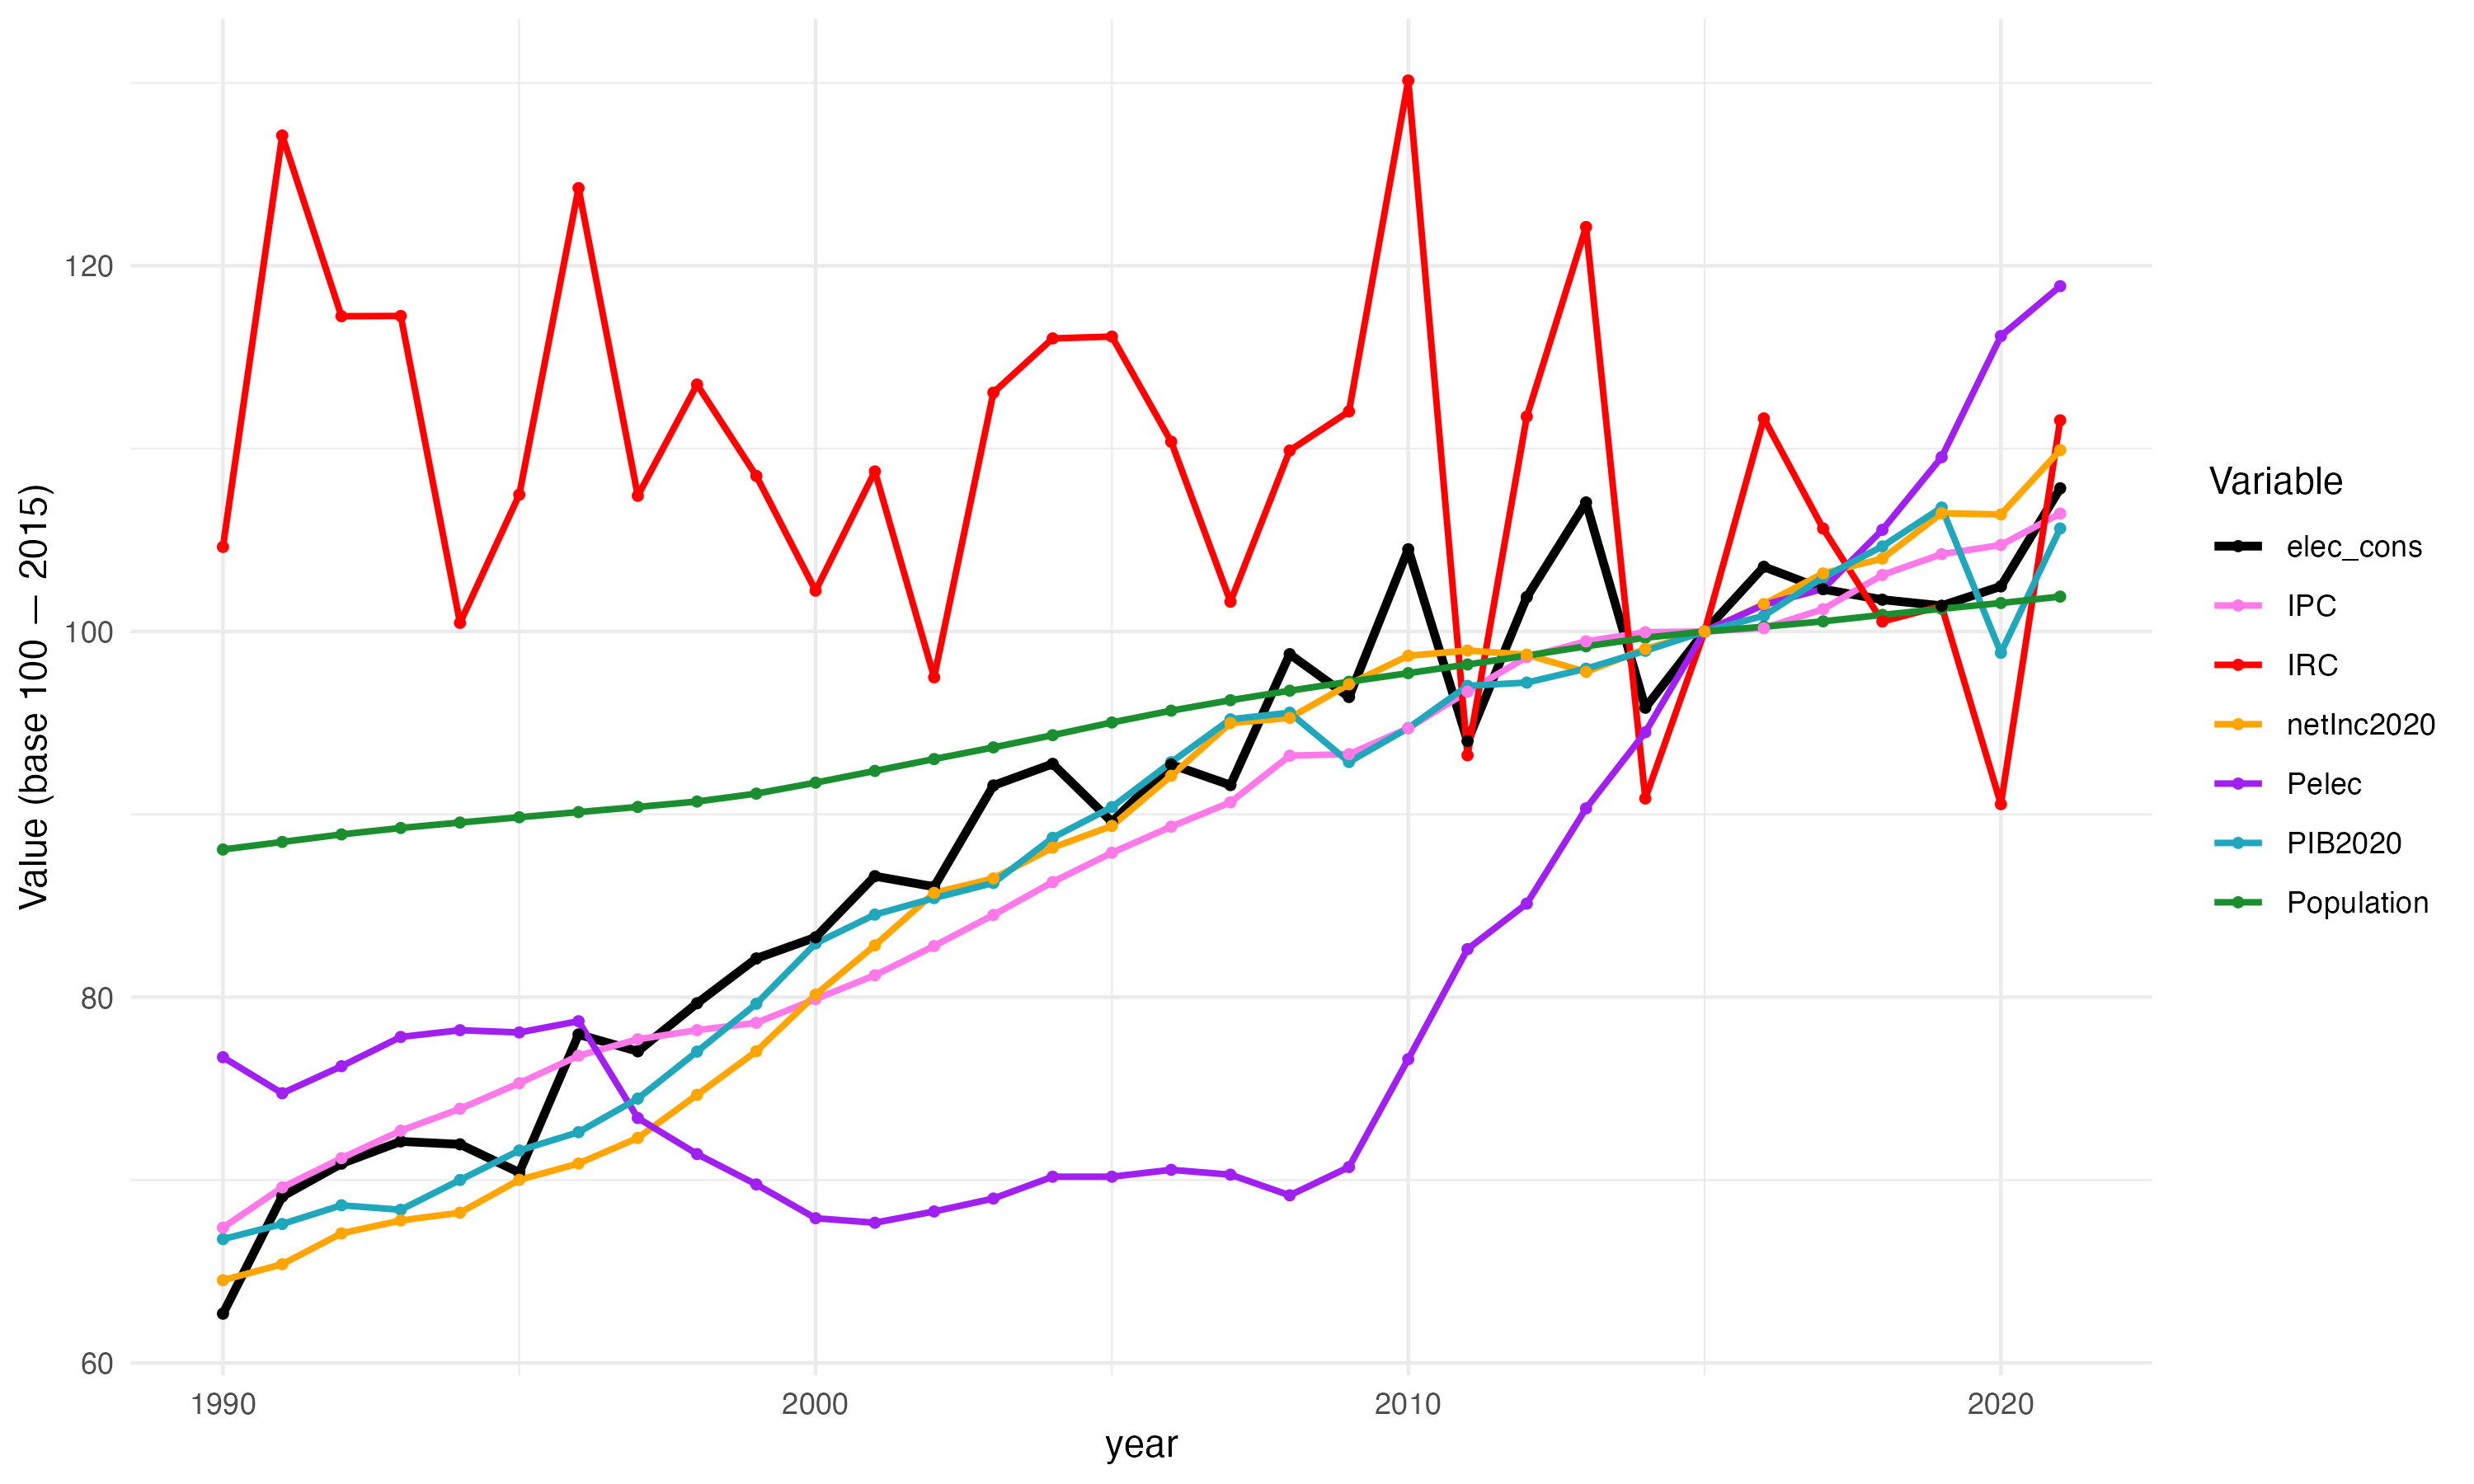
\includegraphics[width=0.5\textwidth]{Images/data_base100_2015.jpeg}
      \caption{Time variation in our data, expressed in base 100 (2015). In black the electricty consumption. In light blue and orange, respectively the GDP and the net disposable income, in euros 2020. In pink, the inflation through CPI, in green the population size. In red the climate index, and eventually in purple the electricity price.}
    \label{var}
  \end{figure}

From figure \ref{var}, we realize how close the GDP and the net disposable income are, only clearly diverging in trend in 2008 and 2020, which we can identify as the 2008 financial crisis and the Covid-19 crisis. Let us note that from 2008, the growth rate of electricity price becomes greather than inflation.

It seems of great matter to take into account the climate variable into our regression model, considering how electricity consumption peaks in cold winters. Eventually, we guess a correlation between the trend decline in the growth rate of electricity consumption and the burst in the price of electricity since 2009. It is likely that this sharp increase is a consequence of the 2008 energy crisis (which might be explained as the interaction of a strong positive demand shock and the ongoing financial crisis\footnote{see \href{https://www.sciencedirect.com/science/article/abs/pii/S0140988319303195}{Balcilar et al. (2020)}}), and the 2005-2008 oil price shock\footnote{see \href{https://www.sciencedirect.com/science/article/abs/pii/S0140988319303195}{Balcilar et al. (2020)}}.

the absolute peak of conventional oil

Choc sur le prix du pétrole en 2008, répercussion sur les prix.\\
Éventuellement effet du marché.

(crise économique ?; mais \textbf{se renseigner aussi sur la mise en place de la libéralisation des prix}\footnote{
    \begin{itemize}
        \item juillet 2007 : éligibilité de tous les consommateurs (dont les clients résidentiels) au marché concurrentiel de l’électricité.
        \item Entrée en vigueur du traité de Lisbonne le 1er décembre 2009.
        \item 7 décembre 2010 : loi NOME (Nouvelle Organisation du Marché de l’Électricité) qui vise à favoriser la concurrence sur le marché de l’électricité (\textit{e.g.} mise en place de l'accès régulé à l'électricité nucléaire historique).
\end{itemize}})

\subsection{Model}
The regression equation \eqref{eq:reg} is a model of electricity consumption seeking to explain the logarithm of per capita electricity consumption by the logarithm of per capita GDP (a proxy for income per capita\footnote{It is however a rough proxy, as the relationship between GDP and household income can be influenced by the division of value between labor and capital, the french tax system and redistribution of wealth, unemployment effects and sectoral effects.
Considering that GDP per capita}) in constant currency and the logarithm of the price of electricity in constant currency. 

\begin{equation} \label{eq:reg}
\ln{\frac{c_{elec}}{pop}} = \alpha + \beta_1 \ln{\frac{{PIB}}{pop}} + \beta_2 \ln{\frac{prix_{elec}}{IPC}} + \beta_3 IRC + \varepsilon
\end{equation}

From an economic point of view, the consumption of a good could be explained by an income effect and a price effect, to which other effects may be added if necessary. Here, we add the Climate Rigor Index (\textit{Indice de Rigueur Climatique}, IRC) to control for climate variation (\textit{e.g.} a colder winter increases electricity consumption).

$\beta_1$ and $\beta_2$ represent respectively the income elasticity and the price elasticity of electricity consumption, \textit{i.e.} the percentage change in electricity consumption in relation, respectively, to a percentage change in income and the percentage change in prices. \\


\section{Results}
